\section[Calcite dissolution and precipitation (1D)]{1D reactive transport: calcite dissolution and precipitation}

\subsection{Definition}
In this example, a one-dimensional column that initially contains
calcite mineral is continuously flushed by water that contains magnesium
chlorine (Fig. \ref{c:cal_dom}). With the movement of water front,
calcite starts to dissolve and dolomite is formed temporarily.
\begin{figure}[!htb]
  \begin{center}
    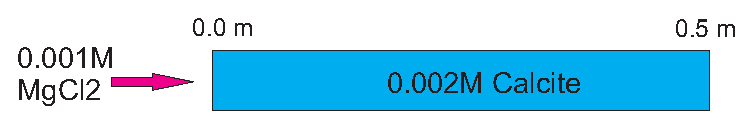
\includegraphics[scale=0.5]{PART_III/HC/calcite_domain.eps}
  \end{center}
  \caption{Model domain}
  \label{c:cal_dom}
\end{figure}
\subsubsection*{Media Properties}
The media properties of this model is listed in Table \ref{tab:c_calcite_mp}.

 \begin{table}[H]
  \begin{center}
  \caption{Material properties} %\footnotesize
  \begin{tabular}{lrl}
\hline\noalign{\smallskip}
  \hline
 Parameter & Value & Unit \\
  \hline
 Column length & $0.5$ & $m$ \\
 Effective porosity & $0.32$ & $-$ \\
 Bulk density & $1.8\times10^{3}$ & $kg \cdot m^{-3}$ \\
 Longitudinal dispersivity & $0.0067$ & $m$ \\
 Pore velocity & $9.375\times10^{-6}$ & $m \cdot sec^{-1}$ \\
 Flow rate & $3\times10^{-6}$ & $m^{3} \cdot sec^{-1}$ \\
  \hline
  \hline
  \end{tabular}
  \label{tab:c_calcite_mp}
  \end{center}
  \end{table}

For OpenGeoSys-GEMIPM2K calculation, all the possible chemical species
need to be explicitly set up for initial and boundary conditions. In
this example, all concentration values are given in the unit of
$mol \cdot kg^{-1}$ water. Detailed values can be get from the *.ic and *.bc files in the corresponding benchmark folder.

\subsection{Solution}
This model can be simulated by \GeoSys-PHREEQC, \GeoSys-ChemApp, and
\GeoSys-GEMIPM2K. In these benchmarks, we use the Nagra/PSI
database \cite{PSI_Database:02}, which provides same thermodynamic
data for all three calculations. Fig. \ref{c:cal_rst}
shows the three simulation results. Solid lines are for \GeoSys-PHREEQC,
symbols "+" are for \GeoSys-GEMIPM2K, and triangles are for \GeoSys-ChemApp.

\begin{figure}[!htb]
  \begin{center}
    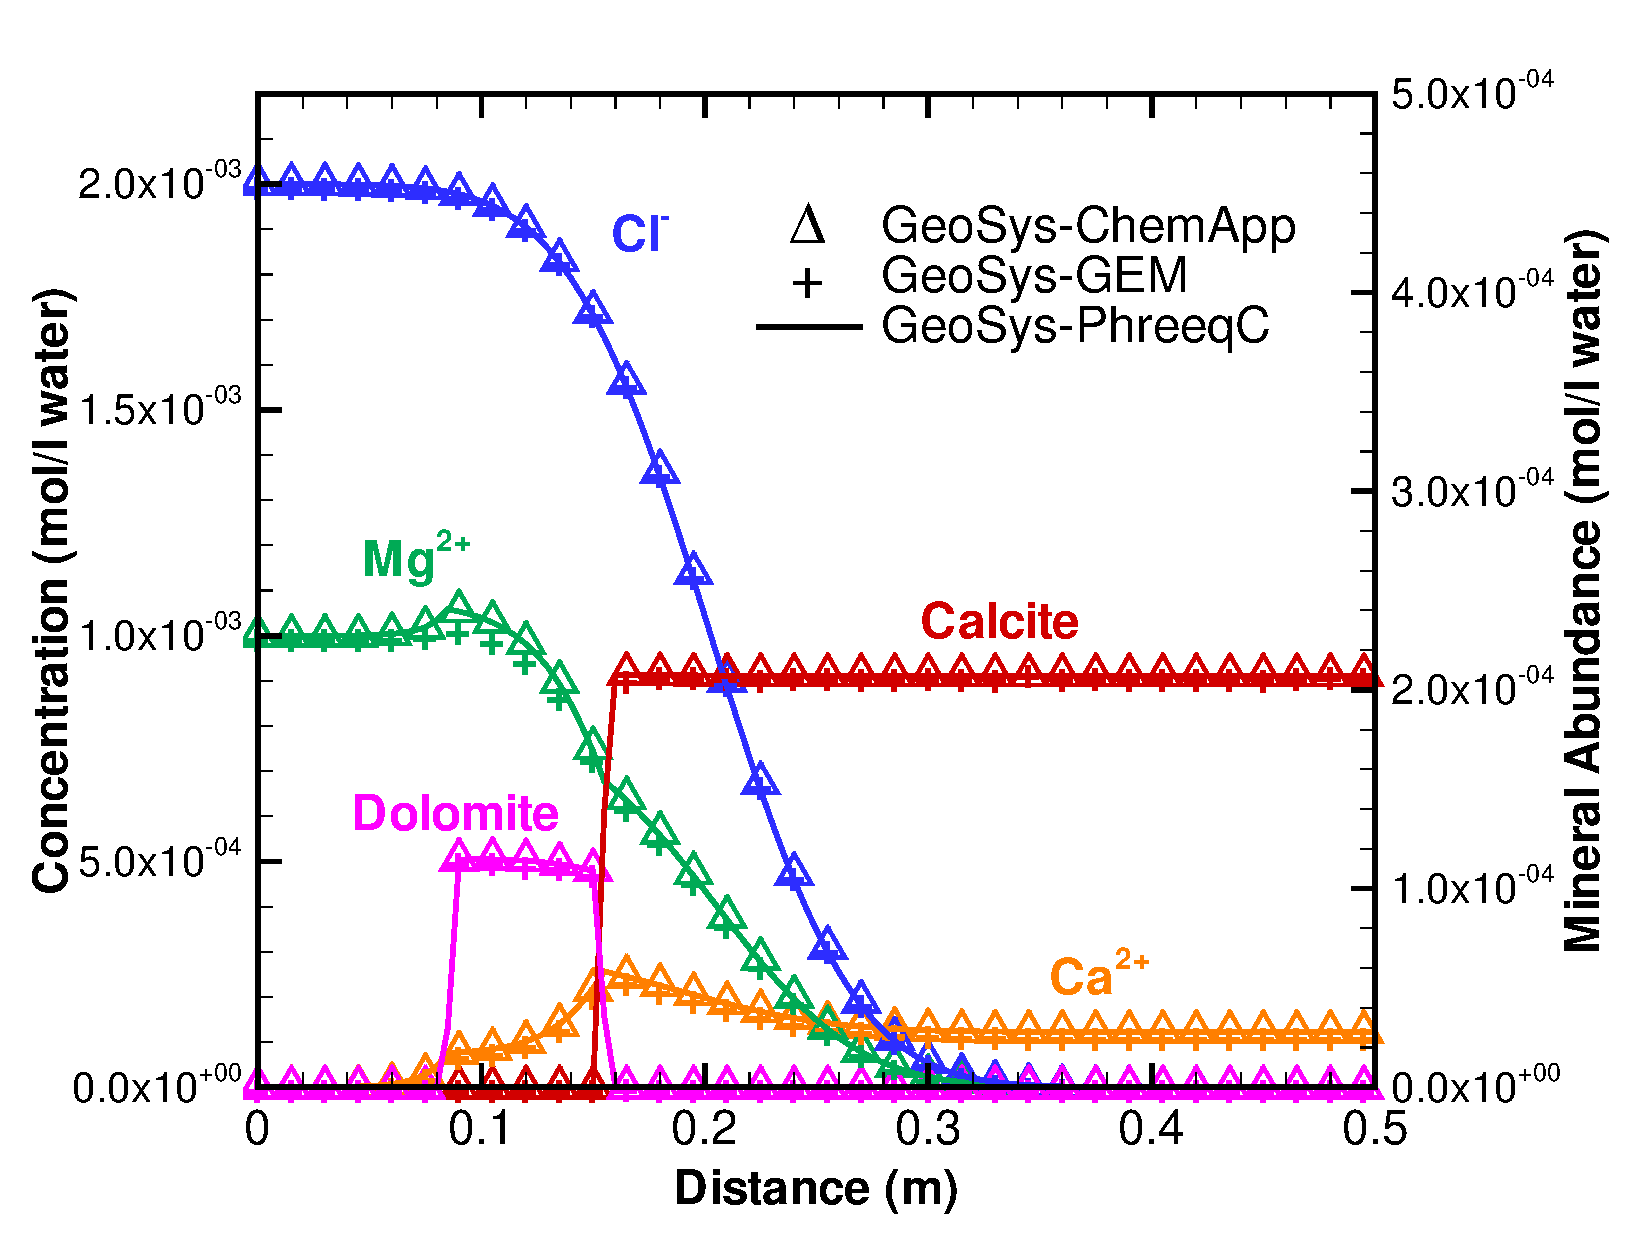
\includegraphics[scale=0.3]{PART_III/HC/calcite_result.eps}
  \end{center}
  \caption{Benchmark results from \GeoSys-ChemApp, \GeoSys-PHREEQC, and \GeoSys-GEMIPM2K}
  \label{c:cal_rst}
\end{figure}
